\chapter{数列和数列求和}

\section{数列的概念}
\subsection{数列的定义}

首先让我们再来看一看人类最先认识的数——自然数:
$1,2,3,4,\ldots,n,n+1,\ldots$, 它们是一串依次排列的
数,从1开始,逐次加1至无穷,这就是本节要讲的数列的
一个原始的例子.下面再举几个数列的例子:

\begin{example}
    在自然数里,把被3整除,被3除余1,被3除
余2的那些数,分别由小到大排列成数列.
\end{example}

\begin{solution}
    被3整除的数:$3,3\x2,3\x3,3\x4,\ldots,3n,3(n+1),\ldots$

被3除余1的数:$3+1,3\x2+1,3\x3+1,3\x4+1,\ldots,3n+1,3(n+1)+1,\ldots$

被3除余2的数:$3+2,3\x2+2,3\x3+2,3\x4+2,\ldots , 3n+2,3(n+1) +2,\ldots$
\end{solution}

\begin{example}
    某人考察,一对兔子经过一年的繁殖,总共可以
有多少对兔子,假设兔子的生殖力是这样的:每一对兔子每
一个月可以生一对兔子,并且兔子在生出两个月以后就具有
生殖后代的能力,在各月份里观察到的兔子的对数如下表所
示:
\begin{center}
\begin{tabular}{c|cccccccccccc}
\hline
$n$&1&2&3&4&5&6&7&8&9&10&11&12\\
\hline
$u_n$&2&3&5&8&13&21&34&55&89&144&233&377\\
\hline
\end{tabular}
\end{center}

设$n$代表月份,$u_n$代表该月内兔子对数.在第一个月里,
第一对兔子生了一对后代,因此$u_1=2$, 在这两对中,只有
第一对能够在下一个月里生一对兔子,所以$u_2=3$, 以后各
月的兔子总对数除了上一个月的兔子总对数外,再加上其中1
能够在这个月产生后代的兔子对数,即前一个月的兔子的总
对数,因此以后各月的兔子总对数可以由公式:
\[u_n=u_{n-1}+u_{n-2},\qquad (2<n\le 12)\]
计算出来.
\end{example}

\begin{example}
    试将$\frac{1}{7}$准确到$\frac{1}{10},\frac{1}{10^2},\frac{1}{10^3},\ldots$
的不足近似值和过剩近似值分别排成数列.
\end{example}

\begin{solution}
    将$\frac{1}{7}$
化成无限循环小数得到
$\frac{1}{7}=0.\dot{1}4285\dot{7}$. 如果
分别按去尾法和进一法舍取近似数,就是说,取$0.\dot{1}4285\dot{7}$前
$n$个数位上的数码而把它后面尾部数码都舍去,这样得到的
有限小数$u_n^-$叫做$\frac{1}{7}$的准确到$\frac{1}{10^n}$
的不足近似值,而把$u_n^+=u_n^-+\frac{1}{10^n}$
叫做$\frac{1}{7}$的准确到$\frac{1}{10^n}$的过剩近似值.

由$\frac{1}{7}$的准确到$\frac{1}{10^n}$的不足近似值组成的数列是
\[0.1,\; 0.14,\; 0.142,\; 0.1428,\; 0.14285,\ldots\]
由$\frac{1}{7}$的准确到$\frac{1}{10^n}$的过剩近似值组成的数列是
\[0.2,\; 0.15,\; 0.143,\; 0.1429,\; 0.14286,\ldots\]
显然有:
\[\begin{split}
   & 0.1<0.14<0.142<0.1428<0.14285<\cdots<\frac{1}{7}\\
   &\qquad <\cdots<
0.14286<0.1429<0.143<0.15<0.2
\end{split}\]
并且
\[\left|u_n^--\frac{1}{7} \right|<\frac{1}{10^n},\qquad \left|u_n^+-\frac{1}{7} \right|<\frac{1}{10^n}\]
\end{solution}

现在我们可以给数列下个定义如下:
\begin{blk}{定义}
    一串依次排列的数$a_1,a_2,\ldots,a_n,\ldots$叫做数列.

    数列中的数,叫做数列的\textbf{项},用$a_n$表示,每一项的位置
序数$n$叫做该项的\textbf{指标},通常写在$a$的右下角,故也叫\textbf{下标}.
数列用符号$\{a_n,\; n=1,2,3,\ldots\}$表示,或简写为$\{a_n\}$.
\end{blk}

依定义,数列就是对每一个自然数$n$指定一项$a_n$, 换言
之,数列就是自然数的函数.

通过前面的例子知道,我们可以用以下几种方式给出一
个数列:
\begin{enumerate}
\item 给出一个以指标$n$表示数列的任意一项$a_n$的公式,
这公式叫做数列的\textbf{通项公式}.例如在例5.1中,数列的通项公
式分别是
\[a_n=3n,\quad b_n=3n+1,\quad c_n=3n+2 \quad (n=1,2,3,\ldots)\]
\item 有的数列从某一项开始能够用在它前面的$k$个项
表示出来.这个表达式,叫做\textbf{递归方程}.例如例5.2中的数列,
由两个初始值$u_1=2$, $u_2=3$和一个递归方程给出:
\[u_n=u_{n-1}+u_{n-2},\qquad (n=3,4,5,\ldots,12)\]
\item 有的数列直接用语言描述它的$a_n$项,用来作一般
性的讨论,如例5.3中的数列.
\end{enumerate}

\subsection{数列的种类及其定义}
\subsubsection{有穷数列和无穷数列}

有末项的数列叫做\textbf{有穷数
列},无末项的数列叫做\textbf{无穷数列}.如例5.2的数列是有穷数
列,例5.1, 例5.3的数列是无穷数列.


\subsubsection{单调数列和摆动数列}

数列$\{a_n\}$中的项,若满足
不等式
\begin{itemize}
    \item $a_{n+1}\ge a_n,\quad (n=1,2,3,4,\ldots,n,\ldots)$, 那么数列
叫做\textbf{不减的}; 
\item 如果$a_{n+1}> a_n,\quad (n=1,2,3,4,\ldots,n,\ldots)$,那么数
列叫做\textbf{递增的};
\item 如果$a_{n+1}= a_n,\quad (n=1,2,3,4,\ldots,n,\ldots)$,那么数
列叫做\textbf{常数列};
\item 如果$a_{n+1}\le a_n,\quad (n=1,2,3,4,\ldots,n,\ldots)$,那么数
列叫做\textbf{不增的};
\item 如果$a_{n+1}< a_n,\quad (n=1,2,3,4,\ldots,n,\ldots)$,那么数
列叫\textbf{递减的}.
\end{itemize}

以上各种数列统称为\textbf{单调数列}.

数列$\{a_n\}$中的项,如果总有一些项大于前面的项,又总
有一些项小于前面的项,那么数列叫做\textbf{摆动数列}.

例如:以下数列都是摆动数列
\begin{itemize}
    \item 数列$\{(-1)^{n+1}\}$:$1,-1,1,-1,\ldots$
    \item 数列$a_n=\begin{cases}
        \frac{1}{n}, & \text{$n$是奇数}\\
        \frac{n}{n+1}, & \text{$n$是偶数}\\
    \end{cases}$:$1,\frac{2}{3},\frac{1}{3},\frac{4}{5},\frac{1}{5},\frac{6}{7},\ldots$
    \item 数列$\{(-1)^{n}n\}$:$-1,2,-3,4,\ldots$
\end{itemize}

\subsubsection{有界数列和无界数列}
有穷数列一定有最大项和最小项,无穷数列就不一定有
此性质.无穷数列可分成有界数列和无界数列.

\begin{blk}{定义}
任何一项的绝对值都小于某一正数,即$|a_n|<M,\quad (M>0)$的数列叫做\textbf{有界数列};没有这样正数存在的数列
叫做\textbf{无界数列}.    
\end{blk}
 
例如,数列$\{(-1)^n\}$和$\{n+(-1)^n n\}$都是无界数列.

数列$\left\{(-1)^{n+1}\left(1+\frac{1}{n}\right)\right\}$
是有界数列,因为
\[|a_n|=\left|(-1)^{n+1}\left(1+\frac{1}{n}\right)\right|=1+\frac{1}{n}\le 2,\quad (n=1,
2,3,4,\ldots)\]

若数列递增,并且所有$a_n\le M$(定数),则称\textbf{数列有上
界}$M$.

\begin{blk}{推论1}
    递增有上界数列一定是有界数列.
\end{blk}

 若数列递减,并且所有$a_n\ge M$(定数),则称\textbf{数列有下
界}$M$.

\begin{blk}{推论2 }
    递减有下界数列一定是有界数列.
\end{blk}

\begin{blk}{推论3}
    有穷数列一定是有界数列.
\end{blk}

图示数列的最简单的方法是直接把点$a_1,a_2,a_3,\ldots$标
在数轴上,这种图象可以清楚地表示数列变化的状态和趋
势.图5.1是几个数列的图象.

\begin{figure}[htp]
    \centering
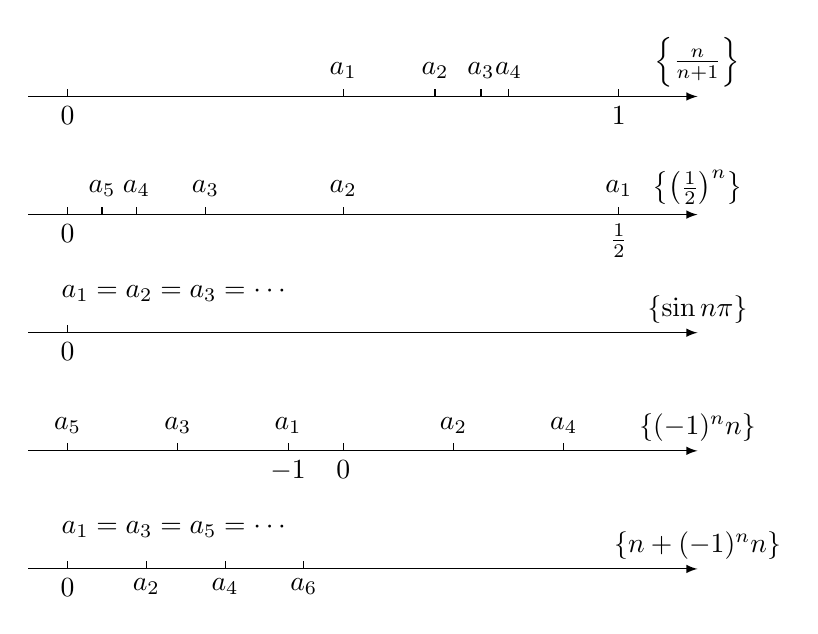
\begin{tikzpicture}[>=latex]
\begin{scope}
    \draw[->] (-0.5,0)--(8,0)node[above]{$\left\{\frac{n}{n+1}\right\}$};
    \foreach \x/\xtext in {{1/2}/a_1, {2/3}/a_2,   {3/4}/a_3,  {4/5}/a_4}
    {
        \draw (\x*7,0)--(\x*7,.1)node[above]{$\xtext$};
    }
\foreach \x in {0,1}
{
    \draw (\x*7,0)node[below]{$\x$}--(\x*7,.1);
}
\end{scope}    
\begin{scope}[yshift=-1.5cm]
    \draw[->] (-0.5,0)--(8,0)node[above]{$\left\{\left(\frac{1}{2}\right)^n\right\}$};   
    \foreach \x/\xtext in {{1/2}/a_1, {1/4}/a_2,   {1/8}/a_3,  {1/16}/a_4, {1/32}/a_5}
    {
        \draw (\x*14,0)--(\x*14,.1)node[above]{$\xtext$};
    }
\foreach \x/\xtext in {0/0,1/\frac{1}{2}}
{
    \draw (\x*7,0)node[below]{$\xtext$}--(\x*7,.1);
}
\end{scope}   
\begin{scope}[yshift=-3cm]
    \draw[->] (-0.5,0)--(8,0)node[above]{$\left\{\sin n\pi\right\}$};
    \draw (0,0)node[below]{0}--(0,.1);
    \node at (-.2,.5)[right]{$a_1=a_2=a_3=\cdots$};
\end{scope}   
\begin{scope}[yshift=-4.5cm]
    \draw[->] (-0.5,0)--(8,0)node[above]{$\left\{(-1)^n n\right\}$};
    \foreach \x/\xtext  in {-5/a_5,-3/a_3,-1/a_1,2/a_2,4/a_4}
{
    \draw (\x*.7+3.5,0)--(\x*.7+3.5,.1)node[above]{$\xtext$};
}
\foreach \x in {-1,0}
{
    \draw (\x*.7+3.5,0)node[below]{$\x$}--(\x*.7+3.5,.1);
}


\end{scope}   
\begin{scope}[yshift=-6cm]
    \draw[->] (-0.5,0)--(8,0)node[above]{$\left\{n+(-1)^n n\right\}$};
    \node at (-.2,.5)[right]{$a_1=a_3=a_5=\cdots$};
    \foreach \x/\xtext  in {0/0, 2/a_2,4/a_4,6/a_6}
{
    \draw (\x*.5,0)node[below]{$\xtext$}--(\x*.5,.1);
}
\end{scope}   
\end{tikzpicture}
    \caption{}
\end{figure}
 

\section*{习题5.1}
\addcontentsline{toc}{subsection}{习题5.1}
\begin{enumerate}
    \item 自然数里的质数由小到大排成一个数列,试依次写出
    它的前10个质数.
    \item 分别用通项公式表示由小到大排列着的偶数数列和奇数数列.
    \item 试写出下列各数列的通项公式
    \begin{multicols}{2}
 \begin{enumerate}
    \item $1^2,\; 2^2,\; 3^2,\; 4^2,\; \ldots$
    \item $1,\; -\frac{1}{2},\; \frac{1}{2}-\frac{1}{3},\; \frac{1}{3}-
    \frac{1}{4},\; \ldots$
    \item $\frac{3}{2},\; \frac{4}{3},\; \frac{5}{4},\; \frac{6}{5},\; \ldots$
    \item $\frac{1\cdot 3}{2\cdot 4},\; \frac{3\cdot 5}{4\cdot 6},\; \frac{5\cdot 7}{6\cdot 8},\; \frac{7\cdot 9}{8\cdot 10},\; \ldots$
     \item $\frac{10}{3},\; \frac{20}{9},\; \frac{30}{27},\; \frac{40}{81},\; \ldots$
     \item $1,\; 1\cdot 2,\; 1\cdot 2\cdot 3,\; 1\cdot 2\cdot 3\cdot 4,\;\ldots $
     \item $-1,\; 1,\; -1,\; 1,\; -1,\; \ldots$
     \item $1,\; -\frac{1}{2},\; \frac{1}{3},\; -\frac{1}{4},\; \frac{1}{5},\; \ldots$
     \item $\frac{1}{1\cdot 2},\; -\frac{1}{3\cdot 4},\; \frac{1}{5\cdot 6},\; -\frac{1}{7\cdot 8},\; \ldots$
\end{enumerate}       
    \end{multicols}

    \item 根据下列各数列的通项公式,写出它的前10项.
 \begin{enumerate}
    \item $a_n=\cos n\pi,\quad (n=1,2,3,\ldots)$
    \item $a_n=\frac{2+(-1)^n}{n},\quad (n=1,2,3,\ldots)$
    \item $f(n)=\begin{cases}
        \frac{1}{n},& \text{$n$为奇数}\\
        \frac{n}{n+1},& \text{$n$为偶数}\\
    \end{cases}$
\end{enumerate}       

\item 试将所有整数排成一个数列,并且用通项公式表示
出来.
\item 数列的通项公式是
\[f(n)=\frac{5+3\sqrt{5}}{10}\left(\frac{1+\sqrt{5}}{2}\right)^n+\frac{5-3\sqrt{5}}{10}\left(\frac{1-\sqrt{5}}{2}\right)^n,\quad (n=1,2,3,\ldots)\]
\begin{enumerate}
    \item 求$f(1)$, $f(2)$;
    \item 求证$f(n)=f(n-1)+f(n-2)$.
\end{enumerate}

\item 判断下列各数列的类型并图示它前5项.
\begin{enumerate}
    \item $a_n=1-2n,\quad (n=1,2,3,\ldots,10)$;
    \item $a_n=\frac{2n+1}{n},\quad (n=1,2,3,\ldots)$;
    \item $a_n=\frac{(-1)^n2^n}{4},\quad (n=1,2,\ldots,5)$;
    \item $a_n=\frac{(-1)^{n+1}n}{n+1},\quad (n=1,2,3,\ldots)$;
    \item $\sqrt{2}$的准确到$1,\; 0.1,\; 0.01,\; \ldots$的过剩近似值.
    \item $a_n=\frac{2+(-1)^n}{n},\quad (n=1,2,3,\ldots)$;
    \item $a_n=(1)^n\left(\frac{n-1}{n+1}\right)^2,\quad (n=1,2,3,\ldots)$;
    \item $a_n=\frac{2n^2-3}{n},\quad (n=1,2,3,\ldots)$;
    \item $a_n=\frac{-2n^2-3}{n},\quad (n=1,2,3,\ldots)$;
    \item $a_n=\tan \frac{n\pi}{3},\quad  (n=1,2,3,\ldots)$.
\end{enumerate}
\item 数列的通项公式是
\[a_n=2n^2-3,\quad (n=1,2,3,\ldots)\]
求数列的第5项,下面三个数:84788、32352和
72197中,哪个数是数列中的项,是第几项?
\end{enumerate}

\section{数列求和举例}
在本节,我们要复习第一册已经学习过的两个简单而重
要的数列,即等差数列和等比数列,同时通过例题来说明几
种常用的求数列前$n$项和的方法.

如果一个数列,从第二项起,每一项减去它的前面的一
项所得的差都等于同一个常数,那么这个数列叫做\textbf{等差数
列},这个常数叫做等差数列的\textbf{公差},用符号$d$表示.等差数
列的通项公式是
\[a_n=a_1+(n-1)d,\qquad (n=1,2,3,\ldots)\]
它的前$n$项求和公式是
\[S_n=\frac{n(a_1+a_n)}{2}\]
或
\[S_n=na_1+\frac{n(n-1)}{2}d\]
我们已在第一册给出上面求和公式的推导过程,现在建议读
者独立地把它们推导出来,在通项公式与求和公式中共包含
了五个数量:$a_1$, $d$, $n$, $a_n$和$S_n$.如果问题给出了其中三个
数量,那么其余两个数量便可由它们解出来.

\begin{example}
    在数轴上有两个点$A(4.5)$和$B(12.5)$, 在其
间插入四个等间隔的点,求这些点的坐标.
\end{example}

\begin{solution}
    在$A$和$B$两点之间插入四个等间隔的点后,这六个
    点的对应坐标成等差数列,

$\because\quad     a_1=4.5,\quad a_6=12.5,\quad n=6$

$\therefore\quad     12.5=4.5+(6-1)d$,解得:$d=1.6$.

所求四个点的坐标分别是
$6.1,\; 7.7,\; 9.3,\; 10.9$.
\end{solution}

\begin{blk}{定义}
    给出两个数,其间插入一个数,使成等差数列,
被插入的数叫做这二数的\textbf{等差中项}.
\end{blk}

\begin{blk}{推论}
    若$a,b,c$三个数成等差数列,则等差中项
\[b=\frac{a+c}{2}\]
\end{blk}
 
事实上,依定义有
\[b-a=c-b\]
移项,得
\[2b=a+c\]
即
\[b=\frac{a+c}{2}\]
    
\begin{example}
    在甲地有48根电杆,从离甲地1000米的地方树立
    第一根电杆,以后每隔15米树立一根电杆,载重汽车每次只
    能拖运三根电杆,问由一辆汽车去完成任务至少需要行驶多
    少公里?
\end{example}

\begin{solution}
    汽车需运电杆$48\div 3=16$次才能完成任务,所以,
    $n=16$.设$a_n$为第$n$次拖运电杆再返回原地所行驶的路程,依
    题意$\{a_n\}$是等差数列,且知
\[    a1=2060,\qquad d=90,\qquad n=16\]
因此:
\[\begin{split}
    S_n&=na_1+\frac{n(n-1)}{2}d\\
    &=16\x 2060+\frac{16\x 15}{2}\x 90\\
    &=43760\text{(米)}=43.76\text{(公里)}
\end{split}\]

答:汽车需行驶43.76公里,才能完成任务.
\end{solution}

如果一个数列,从第二项起,每一项和前面一项的比都
等于一个常数,那么,这个数列叫做\textbf{等比数列}.这个常数叫
做等比数列的\textbf{公比},通常用字母$q$表示.换言之,等比数
列是满足递归关系$a_{n+1}=qa_{n},\quad (n=1,2,\ldots)$的数列.

显然,当$q>0$时,等比数列是单调的.若$q>1$,等
比数列是递增的;若$0<q<1$,等比数列是递减的;若
$q=1$,等比数列是常数列.

当$q<0$时,等比数列是摆动的.

又当$|q|\le 1$时,等比数列是有界的,当$|q|>1$时,
等比数列是无界的.

我们已经知道等比数列的通项公式是
\[a_n=a_1q^{n-1}\qquad (n=1,2,\ldots)\]
它前$n$项和公式是
\[S_n=\frac{a_nq-a_1}{q-1}\]
若$q<1$, 上式改写为
\[S_n=\frac{a_1-a_nq}{1-q}\]
显然,若$q=1$, 则 $S_n=na_1$.

将$a_n=a_1q^{n-1}$代入求和公式中,得到
\[S_n=\frac{a_1(q^n-1)}{q-1}\]

\begin{blk}{定义}
    任给两个数,在其间插入一个数,使成等比数
列,则所插入的数叫做所给两数的\textbf{等比中项}.
\end{blk}

\begin{blk}{推论}
    若$a,b,c$三个数成等比数列,则等比中项$b=\pm\sqrt{ac}$,(或$b^2=ac$).    
\end{blk}

事实上,依定义有$$\frac{b}{a}=\frac{c}{b}$$
因此:$b^2=ac$,或者$b=\pm\sqrt{ac}$.

\begin{example}
    在81和1之间,插入三个实数,使它们和这两个
数成等比数列.
\end{example}

\begin{solution}
    在81和1之间,插入三个数后,1就成为等比数列
的第5项,因此
\[\begin{split}
  a_5=81q^4&=1\\
  (9q^2+1)(9q^2-1)&=0  
\end{split}\]
$\because\quad q$为实数,$\therefore\quad 9q^2+1\ne 0$,由此得:
\[9q^2-1=0\quad \Rightarrow\quad q=\pm\frac{1}{3}\]
故所求三个实数为$27,9,3$或$-27,9,-3$.
\end{solution}


\begin{example}
    已知一个正三角形,边长为$a$,以此正三角形的
高线为边做第二个三角形,依此类推,求前10个正三角形的
面积的和.
\end{example}

\begin{figure}[htp]
    \centering
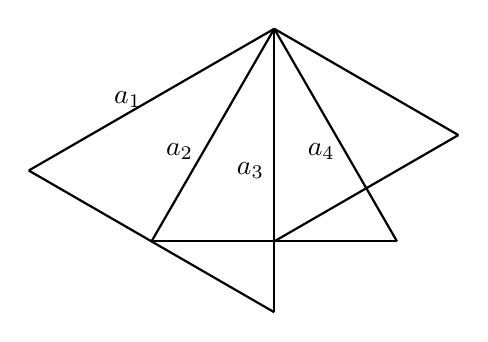
\begin{tikzpicture}[scale=1.8, thick]
    \foreach \x/\xlen in {-150/2, -120/1.732, -90/2, -60/1.732, -30/1.5}
    {
        \draw(0,0)--(\x:\xlen);
    }
\draw (-150:2)--(-90:2); 
\draw (-120:1.732)--(-60:1.732); 
\draw (-90:1.5)--(-30:1.5); 

\foreach \x in {1,2,3,4}
{
    \node at (-180+30*\x:1)[left]{$a_{\x}$};
}
\end{tikzpicture}
    \caption{}
\end{figure}


\begin{solution}
    如图5.2, 设第$k$个这样的正三角形的边长为$a_k$, 高
    为$h_k$, 面积为$A_k,\; (k=1,2,\ldots,10)$, 于是
\[a_1=a,\qquad h_1=\frac{\sqrt{3}}{2}a,\qquad A_1=\frac{1}{2}a_1h_1=\frac{\sqrt{3}}{4}a^2\]
    因为所有正三角形都相似,故对应边与对应高线成比例,即
\[\frac{a_{k+1}}{a_{k}}=\frac{h_{k+1}}{h_k}\]
又依三角形的作法,知
\[a_{k+1}=h_k,\qquad (k=1,2,3,\ldots,10)\]
$\therefore\quad \frac{a_{k+1}}{a_{k}}=\frac{h_{k+1}}{a_{k+1}}=\frac{h_1}{a_1}=\frac{\sqrt{3}}{2}$,

根据相似三角形面积之比等于对应边平方之比,故
\[q=\frac{A_{k+1}}{A_k}=\frac{a^2_{k+1}}{a^2_k}=\left(\frac{a_{k+1}}{a_k}\right)^2=\left(\frac{\sqrt{3}}{2}\right)^2=\frac{3}{4}\]

因此,前10个正三角形面积之和
\[S_{10}=\frac{\frac{\sqrt{3}}{4}a^2\left[1-\left(\frac{3}{4}\right)^{10}\right]}{1-\frac{3}{4}}=\sqrt{3}a^2\left[1-\left(\frac{3}{4}\right)^{10}\right]\]
\end{solution}

为书写简便起见,我们用符号$\displaystyle\sum^n_{i=m}a_i$
表示数列$\{a_i\}$的相邻
的一些项的和.整数$i$在确定了的界限内变动,在$\Sigma$的下
面和上面的数字分别表示求和的起止项的序号,符号“$\Sigma$”
读作sigma.例如
\[\begin{split}
    \sum^n_{i=1}a_i&=a_1+a_2+\cdots+a_n\\
    \sum^n_{i=k}a_i&=a_k+a_{k+1}+\cdots+a_n\\
\end{split}\]

在许多数学问题里,我们需要求出以下标$i$的$k$次多
项式$f(i)$为通项的前$n$项和的公式:
\[S_k(n)=\sum^{n-1}_{i=0}f(i)=f(0)+f(1)+\cdots+f(n-1)\]
这里的指标集是非负整数集.

数列$\{S_k(n)\}$称为数列$\{f(n)\}$的和数列,即
\[\begin{split}
    S_k(1)&=f(0)\\
    S_k(2)&=f(0)+f(1)\\
    S_k(3)&=f(0)+f(1)+f(2)\\
    \cdots&\cdots\cdots
\end{split}\]

为讨论方便起见,规定$S_k(0)=0$, 于是和数列$\{S_k(n)\}$满
足下面两个性质:
\begin{enumerate}
    \item $S_k(0)=0$
    \item $S_k(n+1)-S_k(n)=f(n),\qquad n=0,1,2,\ldots$
\end{enumerate}

我们来考虑这样一个多项式,它在$k$个点$0,1,2,\ldots,
k-1$处与横坐标轴相交,又通过$(k,1)$点,显然这个关于
$n$的多项式为
\[q_k(n)=\frac{n(n-1)\cdots(n-k+1)}{k!}\]
下面来求数列$\{q_k(n)\},\; n=0,1,2,\ldots$的前$n$项和的公式.

\begin{example}
设$q_k(n)=\frac{1}{k!}n(n-1)\cdots(n-k+1)$,则前$n$项的和
\[\begin{split}
    S_k(n)&=\sum^{n-1}_{i=0} q_k(i)=q_k(0)+q_k(1)+\cdots+q_k(n-1)\\
    &=\frac{1}{(k+1)!}n(n-1)\cdots(n-k)
\end{split}\]
换言之,其和是这样一个多项式,它在$0,1,2,\ldots,(k-1)$,共$k$个点处与坐标轴相交且通过$((k+1),1)$点.
\end{example}

\begin{solution}
设$S_k(n)$是一个$n$的$k+1$次多项式,且让$S_k(n)$满
足条件:
\begin{align}
    S_k(0)&=0\\
    S_k(n+1)-S_k(n)&=q_k(n)
\end{align}
由于$q_k(0)=q_k(1)=\cdots=q_k(k-1)=0$, 且
$q_k(k)=1$, 于是
\begin{equation}
    \begin{split}
 S_k(n)&=q_k(0)+q_k(1)+\cdots+q_k(n-1)\\
&=\underbrace{0+0+\cdots+0}_{\text{$k$项}}+1+(k+1)+\\
&\qquad \cdots+
\frac{1}{k!}(n-1)(n-2)\cdots(n-k)     
    \end{split}
\end{equation}

由等式(5.1)和(5.3)得到
\begin{align}
S_k(0)=S_k(1)=\cdots=S_k(k)=0\\
S_k(k+1)=1
\end{align}
从而知道$S_k(n)$有下面$k+1$个因式,即
\[S_k(n)=Cn(n-1)(n-2)\cdots(n-k)\]
这里$C$是未定的常数因子.

常数因子$C$可由(5.5)确定,
\[S_k(k+1)=C(k+1)k(k-1)\cdots2\cdot 1=1\]
$\therefore\quad C=\frac{1}{(k+1)!}$

此处记$(k+1)!=1\cdot 2\cdot 3\cdots k(k+1)$.

因此,
\[\begin{split}
    S_k(n)&=\sum^{n-1}_{i=0} q_k(i)=\sum^{n-1}_{i=0} \frac{1}{k!}i(i-1)\cdots (i-k+1)\\
    &=\frac{1}{(k+1)!}n(n-1)\cdots (n-k)
\end{split}\]
\end{solution}

我们也常用这样一种想法来求数列前$n$项和的公式,即
如果数列的通项能分解成另一个数列相邻两项的差:

$f(n)=F(n+1)-F(n),\; n=0,1,2,\ldots$时,那么前
$n$项的和
\[\begin{split}
   S(n)&= \sum^{n-1}_{i=0} f(i)= \sum^{n-1}_{i=0} [F(i+1)-F(i)]\\
   &=[F(1)-F(0)]+[F(2)-F(1)]+\cdots +[F(n)-F(n-1)]\\
   &=F(n)-F(0)
\end{split}\]


\begin{example}
    求$S(n)=\frac{1}{1\cdot 4}+\frac{1}{4\cdot 7}+\frac{1}{7\cdot 10}+\cdots +\frac{1}{(3n-2)(3n+1)}$的和.
\end{example}

\begin{solution}
$\because\quad \frac{1}{(3i-2)(3i+1)}=\frac{1}{3}\left(\frac{1}{3i-2}-\frac{1}{3i+1}\right)$

当$i=1,2,3,\ldots,n$时,有
\[\begin{split}
    \frac{1}{1\cdot 4}&=\frac{1}{3}\left(\frac{1}{1}-\frac{1}{4}\right)\\
    \frac{1}{4\cdot 7}&=\frac{1}{3}\left(\frac{1}{4}-\frac{1}{7}\right)\\
    \cdots &\cdots\\
    \frac{1}{(3n-2)(3n+1)}&=\frac{1}{3}\left(\frac{1}{3n-2}-\frac{1}{3n+1}\right)
\end{split}\]
因此:
\[\begin{split}
    S(n)&=\sum^n_{i=1}\frac{1}{(3i-2)(3i+1)}\\
    &=\frac{1}{3}\left(\frac{1}{1}-\frac{1}{3n+1}\right)\\
    &=\frac{n}{3n+1}
\end{split}\]
\end{solution}

如果数列的通项是以其它形式的$k$次多项式给出的,我
们可以用待定系数法把它变形为例5.8的形式.


\begin{example}
    求$S_2(n+1)=0^2+1^2+2^2+\cdots+n^2$的和.
\end{example}

\begin{solution}
    设$i^2=\lambda \frac{i(i-1)}{2!}+\mu i,\; (i=0,1,2,\ldots,n)$,由待定系数法求得:
\[\lambda=2,\qquad \mu=1\]
于是:
\[S_2(n+1)=\sum^n_{i=0}i^2=2\sum^n_{i=0}\frac{i(i-1)}{2!}+\sum^n_{i=0}i\]
应用例5.8的结果,得到:
\[\begin{split}
    S_2(n+1)&=2\frac{(n+1)n(n-1)}{3!}+\frac{n(n+1)}{2}\\
    &=\frac{n(n+1)(2n+1)}{6}
\end{split}\]
\end{solution}

\begin{example}
设$a_0,a_1,a_2,\ldots,a_n$成等差数列,求
$S_n=a_0+a_1x+a_2x^2+a_3x^3+\cdots+a_nx^n$的和.    
\end{example}

\begin{solution}
    \begin{equation}
        S_n=a_0+a_1x+a_2x^2+a_3x^3+\cdots+a_nx^n
    \end{equation}
由于(5.6)式中的系数成等差数列,文字$1,x,x^2,\ldots,x^n$成等比数列,利用等差数列的任意相邻的三项有递归关系:
\begin{equation}
    a_n-2a_{n-1}+a_{n-2}=0,\qquad n\ge 2
\end{equation}
知道(5.6)相邻的三项下面等式成立:
\begin{equation}
    a_nx^n-2x(a_{n-1}x^{n-1})+x^2(a_{n-2}x^{n-2})=0,\qquad n\ge 2
\end{equation}
让(5.6)的两边分别乘以$1,2x,x^2$, 然后相加,得
\[\begin{split}
    S_n&=a_0+a_1x+a_2x^2+a_3x^3+\cdots+a_{n-1}x^{n-1}+a_nx^n\\
    -2xS_n&=-2a_0x-2a_1x^2-2a_2x^3-\cdots-2a_{n-1}x^n-2a_nx^{n+1}\\
    x^2S_n&=a_0x^2+a_1x^3+a_2x^4+\cdots+a_{n-1}x^{n+1}+a_nx^{n+2}
\end{split}\]
所以:
\[(1-x)^2 S_n=a_0+(a_1-2a_0)x+0+\cdots+0+(a_{n-1}-2a_n)x^{n+1}+a_nx^{n+2}\]
由(5.8)可知在上面等式中,其余各项为0, 若$x=1$, 两边
除以$(1-x)^2$, 得
\[S_n=\frac{a_0+(a_1-2a_0)x+0+\cdots+0+(a_{n-1}-2a_n)x^{n+1}+a_nx^{n+2}}{(1-x)^2}\]
若$x=1$,原题就变成求等差数列前$n$项的和,这时,
\[S_n=\frac{n(a_1+a_n)}{2}\]
\end{solution}

\begin{example}
    数列$\{v_n\}$由下面递归定义给出:
 \[   v_{n+1}=3v_n-2v_{n-1},\quad v_0=2,\quad v_1=3,\; n=1,2,3,\ldots\]
 求:$v_n$,$S_n=\sum^{n-1}_{i=0}v_i$.
\end{example}

\begin{solution}
    由$v_{n+1}=3v_n-2v_{n-1}$容易看出
  \[  v_{n+1}-v_{n}=2(v_n-v_{n-1})\]
    设$q_n=v_{n+1}-v_n$, $q_{n-1}=v_n-v_{n-1}$, 则$q_n=2q_{n-1},\; (n=1,2,\ldots)$, 换言之,$\{q_n\}$是公比为2的等比数列,
\[\therefore\quad q_n=2q_{n-1}=2^2q_{n-2}=\cdots=2^n(v_1-v_0)=2^n(3-2)=2^n\]
从而:
\[\begin{split}
    q_{n-1}&=v_n-v_{n-1}=2^{n-1}\\
v_n&=(v_n-v_{n-1})+(v_{n-1}-v_{n-2})+\cdots+(v_1-v_0)+v_0\\
&=2^{n-1}+2^{n-2}+\cdots +2+1+2\\
&=(2^n-1)+2=2^n+1\\
\end{split}\]
\[\begin{split}
    S_n=\sum^{n-1}_{i=0}v_i&=\sum^{n-1}_{i=0}(2^i+1)\\
    &=\sum^{n-1}_{i=0}2^i+\sum^{n-1}_{i=0}1\\
    &=(2^n-1)+n=2^n+(n-1)
\end{split}\]
\end{solution}

\section*{习题5.2}
\addcontentsline{toc}{subsection}{习题5.2}
\begin{enumerate}
    \item 在等差数列中
\begin{multicols}{2}
\begin{enumerate}
    \item 若$a_5=100$, $d=\frac{1}{2}$,
    求$a_{100}$;
    \item 若$a_3=-4$, $a_5=2$, 求
    $a_{10}$;
    \item 若$a_p=q$, $a_q=p$, 求$a_{p+q}$;
    \item 用$a_s$, $a_1$, $d$表示$a_n$.
\end{enumerate}
\end{multicols}

\item 在7和35之间插入6个数使它们和已给两数组成等
差数列.
\item 在8和32之间应插入多少个等差中项,可使等差中
项中的前两个数的和与后两个数的和之比为$7:25$.
\item 求证含有奇数个项的等差数列里,第一项,中间
项,最后项也成等差数列.
\item 在三位数里有几个是6的倍数,求它们的和.
\item 求$S_n=1-2+3-4+5-\cdots+(-1)^{n+1}n$的和.
\item 一等差数列前$n$项之和为$S_n=5n^2+3n$, 求$a_n$.
\item 在等差数列中
\begin{enumerate}
    \item 已知$d=2$, $n=15$, $a_{15}=-10$, 求$S_{15}$;
    \item 已知$a_n$, $S_n$和$a_1$,求$d$;
    \item 已知$d$, $S_n$ 和$a_1$,求$n$;
    \item 已知$a_n$, $S_n$和$d$, 求$a_1$.
\end{enumerate}

\item 求等差数列$2\frac{1}{2},1\frac{5}{6},1\frac{1}{6},\ldots$的第$n$项,并求这个等
差级数的最大和.
\item 在等差数列中,若$S_1=a_1+a_3+\cdots+a_{2n-1}=44$,
$S_2=a_2+a_4+\cdots+a_{2n-2}=33$, 求$a_n$.
\item 某化工厂为了加固烟囱,要在烟囱上打32道铁箍,
且使每两道铁箍之间的距离相等,已知最上面一道铁箍处烟
囱的外直径为1.5m,最下面一道箍处烟囱的外直径为3.5m.
求全部铁箍用料的总长.

\item 若$a_1,a_2,\ldots,a_n$成等差数列,求证:
\[\frac{1}{\sqrt{a_1}+\sqrt{a_2}}+\frac{1}{\sqrt{a_2}+\sqrt{a_3}}+\cdots +\frac{1}{\sqrt{a_{n-1}}+\sqrt{a_n}}=\frac{n-1}{\sqrt{a_1}+\sqrt{a_n}}\]

\item 求下列各等比数列的通项公式
\begin{multicols}{2}
\begin{enumerate}
    \item $-1,\;-2,\;-4,\;\ldots$
    \item $\frac{2}{3},\;\frac{1}{2},\;\frac{3}{8},\;\ldots$
    \item $\sqrt{2},\;1,\;\frac{\sqrt{2}}{2},\;\ldots$
    \item $-1,\;1,\;-1,\;\ldots$
    \item $1,\;-\sqrt{\frac{1}{3}},\;\frac{1}{3},\;\ldots$
\end{enumerate}
\end{multicols}

\item 在等比数列里
\begin{enumerate}
    \item $a_1=36$, $a_5=2\frac{1}{4}$,求$q$和$S_5$;
    \item $a_n=1296$, $q=6$, $S_n=625$,求$a_0$和$a_1$;
    \item $a_1=3$, $q=\frac{1}{3}$, $n=8$,求$S_8$;
    \item $S_5=242$, $q=3$,求$a_5$.
\end{enumerate}
\item 在等比数列里,若$a_7-a_5=a_6+a_5=48$, 求$a_1$, $q$和
$S_{10}$.
\item 在160和5之间插入4个数,使这6个数成等比数
列,求这4个数.
\item 求证若$a_1,a_2,\ldots,a_n,\ldots\; (a_i>0,i=1,2,3,
\ldots)$成等比数列,则以下数列均成等比数列:
\begin{multicols}{2}
\begin{enumerate}
    \item $a_1,\; a_3,\; \ldots, a_{2n-1},\; \ldots$;
    \item $ka_1,\; ka_3,\; \ldots, ka_{2n-1},\; \ldots$;
    \item $\frac{1}{a_1},\; \frac{1}{a_2},\; \ldots, \frac{1}{a_{n}},\; \ldots$;
    \item $a^2_1,\; a^2_2,\; \ldots, a^2_{n},\; \ldots$;
    \item $\sqrt{a_1},\; \sqrt{a_2},\; \ldots, \sqrt{a_n},\; \ldots$.
\end{enumerate}
\end{multicols}

\item 从盛满20升纯酒精的容器里倒出一升,然后用水填
满,再倒出一升混合溶液,用水填满,这样继续进行,一共
倒三次,这时容器里有纯酒精多少?
\item 甲厂产量是乙厂产量的40.96\%, 甲厂产品每年增
长的百分率比乙厂产品每年增长的百分率多30\%, 若第四年
甲厂产量和乙厂产量相同,求甲厂每年产品平均增长的百分
率是多少?
\item 一个机器制造厂的原订的三年计划,每年比上一年
增产的机器台数相同,但到了第三年,由于实际需要,须比
原计划多生产1000台,那么每年比上一年的增长百分数就相
同,而且第三年的台数恰为原计划总台数的一半,问实际上
每年生产了多少台?每年比上一年增长的百分数是多少?

\item 某农机厂去年十月份生产拖拉机1000台,这样连同
一月至九月的产量恰好完成全年生产任务,为加速农业机械
化,全厂在年底前又生产了2310台,于是就超额完成全年计
划的21\%.求
\begin{enumerate}
    \item 今年十一,十二月份每月平均增长率;
    \item 今年原计划生产量.
\end{enumerate}

\item 若一个三角形的三个角成等差数列,而它的边成等
比数列,求这个三角形的形状.
\item 已知一个正三角形边长为$a$, 以此正三角形的高线
为边做第二个三角形,依此类推,求前10个正三角形的周长
的和.
\item 求$(x+y)+(x^2+xy+y^2)+(x^3+x^2y+xy^2+y^3)+\cdots$的前$n$项的和.
\item 求$7+77+777+\cdots$的前$n$项的和.

\item 设等比数列$a_1,a_2,\ldots,a_n,\ldots$的公比是$q$.

求证:$a_1a_2\cdots a_n=a^n_1q^{\tfrac{n(n-1)}{2}}$

\item 求下列各数列的和
\begin{multicols}{2}
\begin{enumerate}
    \item $\displaystyle \sum^{n-1}_{i=0} i^3$
    \item $\displaystyle \sum^{n-1}_{i=0} i^4$
    \item $\displaystyle \sum^{n-1}_{i=0} (i-1)i$
    \item $\displaystyle \sum^{n-1}_{i=0} (2i-1)^2$
    \item $\displaystyle \sum^{n-1}_{i=0} \frac{2i+1}{i^2\cdot (i+1)^2}$
\end{enumerate}
\end{multicols}

\item 数列$a_0,a_1,\ldots, a_n,\ldots$中的$a_0,a_1$为已知,且
$a_n=\frac{a_{n-1}+a_{n-2}}{2},\; n=2,3,4,\ldots$, 求$a_n$.

\item 数列$a_1,a_2,\ldots,a_n,\ldots$中,$a_1=2$, 且$a_n=3a_{n-1}+1\; (n=2,3,4,\ldots )$, 求$a_1+a_2+\cdots +a_n$.
\item 已知数列$a_1,a_2,\ldots ,a_n,\ldots$的相邻两项$a_n$,
$a_{n+1}$是方程$x^2+3nx+c_n=0,\; (n=1,2,\ldots)$的两根,当$a_1=
1$时,求$\sum^{2p}_{n=1}c_n$.
\item $n$是非负的整数,试问同时满足下面三个不等式的
整数对$(x,y)$共有多少组?
\[y\ge x,\qquad y\le 3x,\qquad y\le n\]
\item 三角形三条边的长分别是$\ell$, $m$和$n$,这里$\ell$,$m$,
$n$都是正整数,且$\ell\le m\le n$,对于每一个给定的$n$(取
$n=1,2,3,\ldots$),所说的不同形状的三角形有多少个?求
出三角形的个数用$n$表示的一般公式.
\item 数列$\{a_n\}$是:
\[a_1=\frac{1}{3},\qquad \frac{1}{a_{n+1}}-\frac{1}{a_n}=2n+3\quad (n=1,2,3,4,\ldots)\]
\begin{enumerate}
    \item 用3的式子表示一般项;
    \item 用$n$的式子表示前$n$项的和 $\displaystyle\sum^n_{k=1}a_k$
\end{enumerate}

\item 若数列$\{a_n\}$是等差数列,
求证:\[\frac{1}{a_1a_2}+\frac{1}{a_2a_3}+\cdots+\frac{1}{a_{n-1}a_n}=\frac{n-1}{a_1a_n}\]
\end{enumerate}

\section{数学归纳法}
现在我们研究在数学中常用的一种证明方法——数学归
纳法.

我们常常从一些特殊事实归纳出一般结论,这种推理方
法就是通常说的归纳法,用归纳法可以帮助我们从特殊情况
发现一般规律,但如果归纳时所根据的特殊事实没有完全包
括结论中所涉及到的所有情况,结论可能不正确,这就是
说:命题可能对于一系列的特别情形是对的,但是一般并不
正确.

例如,已知函数$f(n)=(n^2-5n+5)^2$,则
\[f(1)=1,\qquad f(2)=1,\qquad f(3)=1,\qquad f(4)=1 \]
如果我们由此得出结论$f(n)=(n^2-5n+5)^2=1$ ($n$是任何自
然数),那就是错误的,事实上,$f(5)=25$, 不等于1.

为了克服这种归纳法的不完全性,我们常采用下述的数
学归纳法来证明一个关于自然数$n$的命题.

数学归纳法的证明逻辑是:

对于一个依赖于自然数$n=1,2,3,\ldots$的命题$p(n)$,如
果
\begin{enumerate}
    \item 当$n=1$时,命题$p(1)$正确;
    \item 假设$n=k,\; (k\ge 1)$时,命题$p(k)$正确,可以
推出$n=k+1$时,命题$p(k+1)$正确,那么,命题$p(n)$对
于一切自然数$n=1,2,3,\ldots$都正确.
\end{enumerate}

这个方法的根据,就是自然数的基本性质:

\begin{blk}{自然数的基本性质}
    令$A$是自然数集$\mathbb{N}$中具有下面性质的子集:
\begin{enumerate}
    \item $1\in A$;
    \item 若$n\in A$,则$n+1\in A$
\end{enumerate}
那么:$A=\mathbb{N}$.
\end{blk}

现在,我们来证明数学归纳法的正确性,设使命题$p(n)$
成立的自然数是自然数集$\mathbb{N}$中的子集$A$, 即$A\subseteq \mathbb{N}$.

根据数学归纳法中的1, $1\in A$; 再根据数学归纳法中
的2,若$n\in A$,则$n+1\in A$.于是,根据自然数的基
本性质,得到
$$A=\mathbb{N}$$
因此,命题$p(n)$对于一切自然数成立.

下面举一些例子说明这个方法的应用.

\begin{example}
    求证:
    \begin{equation}
        1+2+3+\cdots+n=\frac{n(n+1)}{2}
    \end{equation}
\end{example}

\begin{analyze}
    我们注意到和式:$ 1+2+3+\cdots+n$可以递归地定
义为
\[\begin{cases}
    S(1)=1\\
    S(n)=S(n-1)+n,\qquad n=2,3,\ldots
\end{cases}\]
上面的等式为应用数学归纳法去证明打下了基础.
\end{analyze}

\begin{proof}
    \begin{enumerate}
        \item 当$n=1$时,$\because\quad S(1)=1,\quad \frac{1(1+1)}{2}=1$,
        
        $\therefore\quad $等式(5.9)成立.

        \item 假设$n=k,\; (k\ge 1)$时,等式(5.9)成立,即有
\[S(k)=1+2+3+\cdots+k=\frac{k(k+1)}{2}\]
那么,当$n=k+1$时,
\[S(k+1)=1+2+3+\cdots+k+(k+1)=S(k)+(k+1)\]
应用数学归纳法假设于上面的等式,得到
\[\begin{split}
    S(k+1)&=\frac{k(k+1)}{2}+(k+1)=(k+1)\left(\frac{k}{2}+1\right)\\
    &=\frac{(k+1)(k+2)}{2}\\
    &=\frac{(k+1)[(k+1)+1]}{2}
\end{split}\]
即等式(5.9)仍成立.

由所证1和2两步知:
\[1+2+3+\cdots+n=\frac{n(n+1)}{2}\]
对于一切自然数$n$都成立.
\end{enumerate}
\end{proof}

从上例明显地看出,用数学归纳法证明一个命题的步
骤是:
\begin{enumerate}
\item 验证命题$p(n)$, 当$n$取第一个值$n=1$时,$p(1)$正
确.这一条是数学归纳法的基础.
\item 假设当$n=k,\; (k\ge 1)$时,命题$p(k)$正确,证明
当$n=k+1$时,命题$p(k+1)$也正确.这一条是说性质$p(n)$
具有遗传性,可以一代一代地传下去.完成了这两步以后,
就可以断定命题$p(n)$对于一切自然数$n$都正确.因为首先
证明$p(1)$正确,另外由$p(1)$正确推出$p(2)$正确,由$p(2)$正
确推出了$p(3)$正确,依次下去,便可知对于一切自然数$n$,
$p(n)$正确.
\end{enumerate}


有时不一定从1开始,也就是数学归纳法里两句话,可
以改成
\begin{enumerate}
    \item 当$n=k_0$时,命题$p(k_0)$正确.
    \item 从假设$n=k,\; (k\ge k_0)$时,这个命题$p(k)$正确,
    可以推出当$n=k+1$时,这个命题$p(k+1)$也正确,那么$p(n)$
    对于$n\ge k_0$都正确.
\end{enumerate}

\begin{example}
    假设我们只有面额是3分和5分的两种邮票,试证
明可以用面额是3分和5分的两种邮票去付多于7分的任意一
笔邮资.

如果我们对于每一种情形逐一地去证明,譬如,用3分
和5分的邮票各一张可以付8分的邮资;用3分的邮票3张可
以付9分的邮资,用5分的邮票2张可以付10分的邮资等等,
照这样一个一个地验证下去,不是有成效的,因为有无数多
种的情况需要去验证,让我们用数学归纳法来证明.
\end{example}

\begin{proof}
\begin{enumerate}
    \item 我们对于8分的邮资,可以用3分和5分的
    邮票各一张去付,因此,当$n=8$时,命题正确.
    \item 假设用3分邮票和5分的邮票可以付$k$分的邮资,
    我们要证明这两种邮票也可以用来付$k+1$分的邮资.

    因为$k\ge 8$, 有两种可能的情形:$k$分的邮资至少要
    用一张5分的邮票去付;$k$分的邮资完全可以用3分的邮
    票去付.

    在第一种情形下,要付$k+1$分的邮资,只要原来的某一
    张5分的邮票换以两张3分的邮票就可以了;

    在第二种情形下,3分的邮票至少要有3张.要付$k+1$分
    的邮资,只要把原来的三张3分邮票换以两张5分的邮票就可
    以了.

    根据1和2,可以断定$n$为任何大于7的自然数,命
    题正确.
\end{enumerate}


数学归纳法这两步骤,是缺一不可的,从求函数$f(n)=
(n^2-5n+5)^2$的值可知,缺少了步骤2就得出不正确的结
论,同样缺少了步骤1也可能得出不正确的结论.例如,由
于没有验证数学归纳法中的第一条,而得出下面荒谬的结论:
\[2+4+6+\cdots+2n=n^2+n+1\]

我们在下面只证明数学归纳法中的2.

假设$n=k,\; (k>1)$,等式
$2+4+6+\cdots+2k=k^2+k+1$
成立,那么,当$n=k+1$时,
\begin{align*}
    2+4+6+\cdots+2k+2(k+1)&=(2+4+6+\cdots+2k)+2(k+1)\\
&=k^2+k+1+2(k+1)  \tag{数学归纳法假设}\\
&=(k+1)^2+(k+1)+1
\end{align*}
由此知,当$n=k+1$时,等式仍成立.如果仅从数学归纳法
中的2就得出等式对于任何自然数都成立,那是错误的.

事实上,当$n=1$时,等式左边$=2$, 右边$=12+1+1=
3$,因此,上面的等式是错误的.
\end{proof}

\begin{example}
    证明:
\[S(n)=1-2^2+3^2-4^2+\cdots+(-1)^{n-1}n^2=(-1)^{n-1}\frac{n(n+1)}{2}\]
\end{example}

\begin{proof}
\begin{enumerate}
    \item 当$n=1$时,$S(1)=1$,又$(-1)^0\frac{1(1+1)}{2}=1$,所以等式成立.

\item 假设$n=k$时,有
\[S(k)=1-2^2+3^2-4^2+\cdots+(-1)^{k-1}k^2=(-1)^{k-1}\frac{k(k+1)}{2}\]
那么,当$n=k+1$时,有    
\[\begin{split}
    S(k+1)=S(k)+(-1)^k(k+1)^2&=(-1)^{k-1}\frac{k(k+1)}{2}+(-1)^k(k+1)^2\\
    &=(-1)^k(k+1)\left[-\frac{k}{2}+(k+1)\right]\\
    &=(-1)^k \frac{(k+1)(k+2)}{2}\\
    &=(-1)^k \frac{(k+1)[(k+1)+1]}{2}
\end{split}\]
\end{enumerate}

由1和2知,等式对于一切自然数$n$都成立.
\end{proof}


\begin{example}
证明:
\[\begin{split}
    S(n)&= \sin \alpha+\sin (\alpha+\beta)+\sin (\alpha+2 \beta)+\cdots+\sin (a+(n-1) \beta) \\
&= \frac{\sin \frac{n \beta}{2}}{\sin \frac{\beta}{2}} \sin \left(\alpha+\frac{n-1}{2} \beta\right)
\end{split}\]
\end{example}

\begin{proof}
\begin{enumerate}
    \item 当$n=1$时,
\[\because\quad \text{左边}=S(1)=\sin\alpha,\qquad \text{右边}=\frac{\sin\frac{\beta}{2}}{\sin\frac{\beta}{2}}\sin(\alpha+0\cdot \beta)=\sin\alpha\]
$\therefore\quad $等式成立.

\item 假设 $n=k$ 时,
\[\begin{split}
    S(k)&=\sin \alpha+\sin (\alpha+\beta)+\sin (\alpha+2 \beta)+\cdots+\sin (\alpha+(k-1) \beta) \\
&=\frac{\sin \frac{k \beta}{2}}{\sin \frac{\beta}{2}} \sin \left(a+\frac{k-1}{2} \beta\right)
\end{split}\]
成立,那么:
\[\begin{split}
    S(k+1)&= S(k)+\sin(\alpha+k\beta)\\
    &=\frac{\sin \frac{k \beta}{2}}{\sin \frac{\beta}{2}} \sin \left(a+\frac{k-1}{2} \beta\right)+\sin(\alpha+k\beta)\\
    &=\frac{1}{\sin \frac{\beta}{2}}\left[\sin\left(\alpha+\frac{k-1}{2}\beta\right)\sin\frac{k\beta}{2}+\sin(\alpha+k\beta)\sin\frac{\beta}{2}\right]\\
    &=\frac{1}{2\sin \frac{\beta}{2}}\left[\cos\left(\alpha-\frac{\beta}{2}\right)-\cos\left(\alpha+k\beta-\frac{\beta}{2}\right)\right. \\
    &\qquad \qquad \left. +\cos\left(\alpha+k\beta -\frac{\beta}{2}\right)-\cos\left(\alpha+k\beta+\frac{\beta}{2}\right)\right]\\
    &=\frac{1}{2\sin \frac{\beta}{2}}\left[\cos\left(\alpha-\frac{\beta}{2}\right)-\cos\left(\alpha+k\beta+\frac{\beta}{2}\right)\right]
\end{split}\]
\[\begin{split}
    S(k+1)&= \frac{(-2)}{2\sin \frac{\beta}{2}}\sin\left(\frac{2\alpha+k\beta}{2}\right)\sin\left(\frac{-k\beta-\beta}{2}\right)\\
    &=\frac{1}{\sin \frac{\beta}{2}}\cdot \sin\left(\alpha+\frac{k}{2}\beta\right)\cdot \sin\frac{(k+1)\beta}{2}\\
    &=\frac{\sin \frac{(k+1)\beta}{2}}{\sin \frac{\beta}{2}}\sin\left[\alpha+\frac{(k+1)-1}{2}\beta\right]\\
\end{split}\]
即当$n=k+1$时,等式仍成立.由1和2可知,等式
对任何自然数$n$都成立.
\end{enumerate}
\end{proof}

\begin{example}
    用数学归纳法证明,如果$n$是一个正整数,那么
    $x^{2n}-y^{2n}$能被$x+y$整除.
\end{example}

\begin{proof}
\begin{enumerate}
    \item 当$n=1$时,$x^2-y^2=(x+y)(x-y)$能被
    $x+y$整除.
    \item 假设当$n=k$, ($k$是自然数),$x^{2k}-y^{2k}$能被$x+y$
    整除,那么当$n=k+1$时,
\[\begin{split}
    x^{2(k+1)}-y^{2(k+1)}
    &=x^2\cdot x^{2k}-y^2\cdot y^{2k}\\
    &=x^2\cdot x^{2k}-x^2y^{2k}+x^2y^{2k}-y^2\cdot y^{2k}\\
    &=x^2(x^{2k}-y^{2k})+(x^2-y^2)\cdot y^{2k}
\end{split}\]
    
    因为$x^{2k}-y^{2k}$与$x^2-y^2$都能被$x+y$整除,所以$x^2(x^{2k}-y^{2k})+(x^2-y^2)y^{2k}$也能被$x+y$整除,这就是说,$x^{2k+1}-y^{2k+1}$能
    被$x+y$整除.
\end{enumerate}  

根据1和2, 命题成立.
\end{proof}

\begin{example}
    平面上有$n$条直线,其中任何两条不平行,任何
三条不过同一点,证明这$n$条直线把平面分成$f(n)=\frac{1}{2}
(n^2+n+2)$个部分.
\end{example}

\begin{proof}
\begin{enumerate}
    \item 当$n=1$时,直线把平面分成两部分(为了
    简单起见,也说分成两块),又
  \[  f(1)=\frac{1}{2}(1^2+1+2)=2\]
    因此,$n=1$时命题成立.
   \item 假设$n=k$时命题成立,就是
\[f(k)=\frac{1}{2}(k^2+k+2)\]

我们要设法找出$f(k+1)$与$f(k)$的递归关系,即由
$f(k)$求得$f(k+1)$的关系.为此,我们在平面上再增加
一条直线$\ell$(图5.3),因为已知任何两条直线不平行,所以直
线$\ell$与平面上的原$k$条直线都相交,而且这$k$个交点互不相
同,否则与任何三条直线不过同一点的已知条件矛盾,这$k$
个交点将直线$\ell$分成$k+1$段,因此直线$\ell$越过原来的$k+1$
块平面部分,直线上的每段将它所在的原平面块分成两块,
因此要给原来的平面部分的总数$f(k)$增加$k+1$块新的平面
部分,就是
\[f(k+1)=f(k)+(k+1)\]
将$f(k)=\frac{1}{2}(k^2+k+2)$代入上式,得到
\[\begin{split}
    f(k+1)&=\frac{1}{2}(k^2+k+2)+(k+1)\\
    &=\frac{1}{2}(k^2+3k+4)\\
    &=\frac{1}{2}[(k+1)^2+(k+1)+2]
\end{split}\]
这就是说,当$n=k+1$时,命题也成立.

\begin{figure}[htp]
    \centering
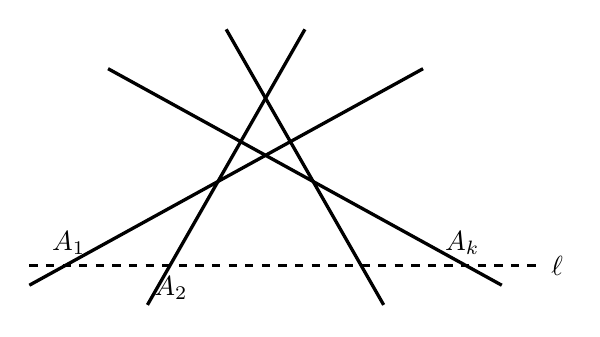
\begin{tikzpicture}[very thick]
    \draw (1.5,-1)--(-.5,2.5);
\draw (-1.5,-1)--(.5,2.5);
\draw (-3,-.75)--(2,2);
\draw (3,-.75)--(-2,2);

\node at (-2.5,-.5) [above] {$A_1$};
\node at (-1.2,-.5) [below] {$A_2$};
\node at (2.5,-.5) [above] {$A_k$};

\draw[dashed, thick] (-3,-.5)--(3.5,-.5)node[right]{$\ell $};

\end{tikzpicture}
    \caption{}
\end{figure}


根据1和2,可知命题成立.
\end{enumerate}
\end{proof}

同学也许会问:例5.18的结果是怎样发现的?数学归纳法
能解决这个问题吗?其实此题的证明已经解决了这个问题,
因为我们证明了$f(n)$可以递归地定义为
\[\begin{cases}
    f(1)=2\\
    f(k+1)=f(k)+(k+1),\qquad k=1,2,\ldots,(n-1)
\end{cases}\]
首先$f(1)$有定义,其次如果知道了$f(1)$, 就知道$f(2)$,
依次推下去,就知道$f(n)$.所以
\[\begin{split}
  f(n)&=[f(n)-f(n-1)]+[f(n-1)-f(n-2)]+\cdots +[f(2)-f(1)]+f(1)\\
  &=n+(n-1)+\cdots +2+2\\
  &=[n+(n-1)+(n-2)+\cdots +2+1]+1\\
  &=\frac{n(n+1)}{2}+1=\frac{n^2+n+2}{2}  
\end{split}\]

\section*{习题5.3}
\addcontentsline{toc}{subsection}{习题5.3}
\begin{enumerate}
    \item 用数学归纳法证明下列各等式:
\begin{enumerate}
    \item $\displaystyle\sum^n_{k=1}3^{k-1}=\frac{3^n-1}{2}$
    \item $\displaystyle\sum^n_{k=1}k(k+1)=\frac{1}{3}n(n+1)(n+2)$
    \item $\displaystyle\sum^n_{k=1}\frac{1}{k(k+1)}=\frac{n}{n+1}$
    \item \[ \begin{split}
      & \cos\alpha+\cos(\alpha+\beta)+\cos(\alpha+2\beta)+\cdots+\cos[\alpha+(n-1)\beta]\\
      &\qquad =\frac{\sin\frac{n\beta}{2}}{\sin\frac{\beta}{2}}\cos\left(\alpha+\frac{n-1}{2}\beta\right)
    \end{split}\]
\end{enumerate}

\item 用数学归纳法证明:
\begin{enumerate}
\item 当$n$是正整数时,$x^n-y^n$能被$x-y$整除.
\item 当$n$是正奇数时,$x^n+y^n$能被$x+y$整除.
\item $(3n+1)7^n-1$能被9整除.
\item 连接的三个自然数的立方和,必定能被9整除.
\item 当$n$是正整数时,$(11)^{n+2}+(12)^{2n+1}$能被133
整除.
\item 当$n$是正整数时,$3^{2n+2}-8n-9$能被64整除.
\end{enumerate}

\item 数列$\{a_n\}$是这样确定的:
\[a1=1,\quad 4a_ka_{k+1}=(a_k+a_{k+1}-1)^2,\quad a_k<a_{k+1}\quad (k=1,2,3,\ldots)\]
\begin{enumerate}
    \item 求 $a_2,a_3,a_4$, 并由此推断$a_n$;
    \item 用数学归纳法证明(a)中推断出的$a_n$的正
确性.
\end{enumerate}

\item 空间有$n$个平面,其中没有两个平面平行,没有三
个平面相交于同一条直线,也没有四个平面过同一个点.

求
证:它们把空间分成$f(n)=\frac{1}{6}
(n^3+5n+6)$份.
\item 有$n$个圆,其中每两个圆都相交于两点,并且每三
个圆不相交于同一点.

求证:这$n$个圆把平面分成$n^2-n+2$
部分.

\item 若数列$\{a_n\}$,当$n\ge 3$时,满足条件
\[\frac{1}{a_1a_2}+\frac{1}{a_2a_3}+\frac{1}{a_3a_4}+\cdots+\frac{1}{a_{n-1}a_n}=\frac{n-1}{a_1a_n}\]
用数学归纳法证明数列$\{a_n\}$是等差数列.
\end{enumerate}
